\section{CPU, Scheduling, and OS Services}
In this section, we will measure the overhead of procedure call, system call, and the time of task creation and context switching.

\subsection{Procedure Call}
First we need to define the overhead of procedure call. We assert that the overhead of function calls stems from three key factors: 1. Preparation of function parameters; 2. The setup of the function's stack frame during the function call; 3. Function return. Considering the code in \ref{lst1}. 
\lstinputlisting[language=C++,label=lst1,caption={Non inline procedure call}]{sourcecode/CPU-Schedule-OS/lst1.c}
In System V AMD64 ABI \textbf{(todo: cite)}, when calling function, the caller needs to setup the arguments for the callee, then pushes the return address and stack base pointer to the stack and jumps to the callee. When callee returns to the caller it will recover the previous stack frame and pop the return address to the program counter register to back to the caller's code. Thus, we can define the overhead of a procudure call as the additional cost incurred by three components: parameter preparation, stack frame adjustment before the jump, and stack frame adjustment upon return. To measure this overhead, we can calculate the time it takes from invoking a simplest function to its return.
\lstinputlisting[label=lst2,caption={Simplest function takes only one argument}]{sourcecode/CPU-Schedule-OS/simplest_func.asm}
By using the simplest function in \ref{lst2}, we can eliminate the performance impact brought about by compiler optimizations (e.g. inlining) and security features (e.g. stack canaries).

Before measuring procedure calls, we also need to figure out the calling conventions. In System V AMD64 ABI, Programs typically pass parameters as table \ref{table:calling-convention-reg}\footnote{We are using cdecl calling convention.}.
\begin{table}[h]
	\centering
	\begin{tabular}{c|c}
		\hline
		\bf{Arguments} & \bf{How they are passed} \\ \hline
		
		First 6 Integers & RDI, RSI, RDX, RCX, R8, R9 \\ \hline

		First 8 Floating Points & XMM0-XMM7 \\ \hline
		
		Others & Stack \\ \hline
	\end{tabular}
	\caption{\textbf{Arguments Passing in System V AMD64 Calling Convention.}}
	\label{table:calling-convention-reg}
\end{table}
From this, we can make an early prediction that, for procedure calls with integer parameters, there won't be a significant difference in calling overhead when the number of parameters is less than or equal 6. It's only when there are more than 6 parameters that significant differences may arise due to memory writes.

\paragraph{Measure the overhead.} To measure the overhead more precisely, we use \texttt{rdtscp}\footnote{In order to preserve the execution order, we use \texttt{rdtscp} instead of \texttt{rdtsc}} instruction \textbf{(todo: cite)} to read from the processor’s time-stamp counter in order to get the number of CPU cycles. In order to mitigate the impact of process scheduling, we call the same function consecutively multiple times. Also, we use \texttt{setpriority()} to raise the scheduling priority of our testing program. Before conducting the tests, we ensure that the size of the test program is smaller than a page and disable swap. This is done to maximize the likelihood of the program being fully loaded into memory during the testing process. Every testing procedure call will be executed 0x1000000 times. The result is listed in table \ref{table:procedure-test}
\begin{table}[h]
	\centering
	\begin{tabular}{c|c}
		\hline
		\bf{Arguments} & \bf{Average Cycles} \\ \hline
		0 & 50.617 \\ \hline
		1 & 50.971 \\ \hline
		2 & 47.398 \\ \hline
        3 & 50.075 \\ \hline
        4 & 52.003 \\ \hline
        5 & 51.180 \\ \hline
        6 & 49.692 \\ \hline
        7 & 57.141 \\ \hline
	\end{tabular}
	\caption{\textbf{Average Cycles of Procedure Call.}}
	\label{table:procedure-test}
\end{table}
Also we remove the function calling to measure the overhead of rdtscp.
The average cycles is $45.260$. This aligns closely with our previous predictions: when the number of parameters is between 0 and 6, there is no significant difference in overhead. It is only when memory access is required that a noticeable increase in overhead becomes apparent.

\textbf{todo: more precisely measure this by sub the time spent in kernel mode.}

\subsection{System Call}
The overhead of a syscall, as compared to a regular procedure call, primarily arises from the context switching. Therefore, our primary task is to ascertain when will syscalls, or more frequently encountered libc syscall wrappers for usermode programmers, genuinely trap into kernel mode.

\paragraph{Virtual Syscall.} Virtual Dynamic Shared Object, vDSO is a kernel mechanism for exporting a selected part of kernel space routines to user space. VDSO provides user mode programs with vsyscalls. These virtual syscalls eliminate the need for user mode programs to spend time on context switching for certain simple syscalls. They are the syscalls without really trapping into kernel.

\begin{lstlisting}[caption=vDSO mapping]
gef> vmmap
...
0xffffffffff600000 
0xffffffffff601000 
0x0000000000000000 --x [vsyscall]
\end{lstlisting}

\paragraph{Measure the overhead.} We choose a simple system, clock\_gettime() to measure the overhead. Since we have the vDSO mapping, subtracting the number of cycles required for a syscall from those needed for VDSO can provide an estimate of the overhead associated with context switching. The result is in table \textbf{(todo: test with BPF or add a new syscall to kernel to measure it more precisely)}.
\begin{table}[h]
	\centering
	\begin{tabular}{c|c}
		\hline
		\bf{syscall} & \bf{vDSO call} \\ \hline
        1517.221 & 63.588 \\ \hline
	\end{tabular}
	\caption{\textbf{Result of Overhead of System Call.}}
	\label{table:procedure-test}
\end{table}
Thus the overhead of syscall can be calculated as follows:
\begin{equation}
    t_{\text{overhead}}=t_{\text{syscall}}-t_{\text{vDSO}}=1453.633\ \text{Cycles}
\end{equation}

\subsection{Task Creation} There are two main approaches to create a new task: \texttt{fork()} and \texttt{pthread\_create()}. Before we measure the task creation time, we should dive deeper into how these two APIs work\footnote{We are using GNU LIBC 2.38.}.

\paragraph{fork() vs. pthread\_create().} Before actually launching a task, both of these functions perform a substantial amount of preparatory work. For now, let's set aside these preparations and focus on how they each initiate a new task. Figure \ref{fig:fork-callstack} shows the call stack when calling \texttt{fork()}
\begin{figure}[htbp]
    \centering
    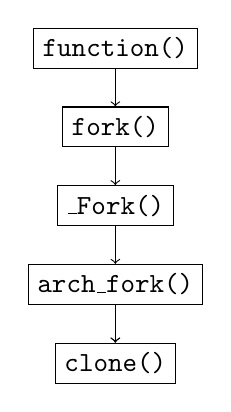
\begin{tikzpicture}[node distance=15pt]
        \node[draw] at(0, 7) (l0) {\texttt{function()}};
        \node[draw] at(0, 6) (l1) {\texttt{fork()}};
        \node[draw] at(0, 5) (l2) {\texttt{\_Fork()}};
        \node[draw] at(0, 4) (l3) {\texttt{arch\_fork()}};
        \node[draw] at(0, 3) (l4) {\texttt{clone()}};
        \draw[->] (l0)  -- (l1);
        \draw[->] (l1)  -- (l2);
        \draw[->] (l2)  -- (l3);
        \draw[->] (l3)  -- (l4);
        \draw[->] (l3)  -- (l4);
    \end{tikzpicture}
    \caption{Call Stack of \texttt{fork()}}
    \label{fig:fork-callstack}
\end{figure}
Figure \ref{fig:pthread-callstack} show the call stack when a program call \texttt{pthread\_create()} on a system that supports \texttt{clone3} syscall\footnote{Firgure 1 shows the function names instead of the versioned symbols.}.
% \lstinputlisting{assets/code/bt.c}
\begin{figure}[htbp]
    \centering
    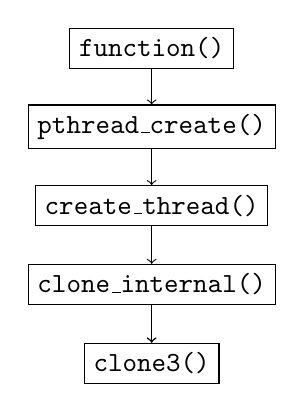
\begin{tikzpicture}[node distance=15pt]
        \node[draw] at(0, 7) (l0) {\texttt{function()}};
        \node[draw] at(0, 6) (l1) {\texttt{pthread\_create()}};
        \node[draw] at(0, 5) (l2) {\texttt{create\_thread()}};
        \node[draw] at(0, 4) (l3) {\texttt{clone\_internal()}};
        \node[draw] at(0, 3) (l4) {\texttt{clone3()}};
        \draw[->] (l0)  -- (l1);
        \draw[->] (l1)  -- (l2);
        \draw[->] (l2)  -- (l3);
        \draw[->] (l3)  -- (l4);
        \draw[->] (l3)  -- (l4);
    \end{tikzpicture}
    \caption{Call Stack of \texttt{pthread\_create()}}
    \label{fig:pthread-callstack}
\end{figure}
After calling \texttt{clone()} and \texttt{clone3()} a new task is created.
We should focus on the these two syscalls which do the job of creating a new thread. 
% \lstinputlisting{assets/code/pthread_cloneflag.c}
Compared to clone, clone3 provides more granular control over the creation of a new process.

\paragraph{Measure.} In order to more accurately measure task creation time and the differences between these two system calls, we conducted separate tests on the distinctions between them. To achieve this, we apply inline hooks to the GNU LIBC library. Before executing syscall, the library function will first jump to our measurement function and save the current CPU cycle. After syscall, it will jump to our measurement function again to calculate the cycles again. \textbf{todo: hook in kernel space, or reimplement fork() and pthread\_create() and then syscall by ourselves}